%!TeX root=../tese.tex
%("dica" para o editor de texto: este arquivo é parte de um documento maior)
% para saber mais: https://tex.stackexchange.com/q/78101

\chapter{Implementações já existentes}

Este capítulo da monografia realizará a análise de implementações de código aberto já existentes de protocolos descentralizados de envio de mensagens. Essas implementações fornecem uma base para compreender os desafios práticos, as abordagens de arquitetura e as estratégias de mitigação de problemas que foram desenvolvidas e testadas pela comunidade. Os protocolos analisados foram selecionados por serem abertos, descentralizados, e por terem uma arquitetura de rede singular, sendo relevante para este estudo. Os protocolos analisados foram categorizados pela sua arquitetura de rede, e divididos em quatro grupos principais: federados, \textit{peer-to-peer} com \textit{relays} que usam \textit{Tor}, \textit{peer-to-peer} com \textit{relays} que não usam \textit{Tor}, e \textit{peer-to-peer} sem \textit{relays}.

Os protocolos analisados federados são:
\begin{itemize}
  \item \href{https://matrix.org/}{\textit{Matrix}}
  \item \href{https://xmpp.org/}{\textit{XMPP}}
  \item \href{https://datatracker.ietf.org/doc/html/rfc5321}{\textit{E-Mail}}
\end{itemize}

Os protocolos analisados \textit{peer-to-peer} com \textit{relays} que não usam \textit{Tor} são:
\begin{itemize}
  \item \href{https://simplex.chat/}{\textit{SimpleX}}
  \item \href{https://datatracker.ietf.org/doc/html/rfc2810}{\textit{IRC}}
  \item \href{https://lora-alliance.org/}{\textit{LoRaWan}}
\end{itemize}

Os protocolos analisados \textit{peer-to-peer} com \textit{relays} que usam \textit{Tor} são:
\begin{itemize}
  \item \href{https://cwtch.im/}{\textit{Cwtch}}
  \item \href{https://ricochet.im/}{\textit{Ricochet}}
  \item \href{https://briarproject.org/}{\textit{Briar}}
\end{itemize}

Os protocolos analisados \textit{peer-to-peer} sem \textit{relays} são:
\begin{itemize}
  \item \href{https://scuttlebutt.nz/}{\textit{Secure Scuttlebutt}}
  \item \href{https://tox.chat/}{\textit{Tox}}
  \item \href{https://bitmessage.org/}{\textit{Bitmessage}}
\end{itemize}

A análise de cada protocolo é focada na arquitetura de rede e não considera em detalhes outras funcionalidades, como chamadas de voz, videoconferência ou compartilhamento de arquivos. A seguir, são apresentadas as análises dos protocolos selecionados.

\section{Protocolos Federados}

Na arquitetura federada de envio de mensagens, cada usuário escolhe um servidor para ser seu provedor de mensagens. Essa máquina será responsável por rotear todas as comunicações do usuário e, em alguns casos, também armazenar suas mensagens. É importante que o usuário possa confiar em seu provedor de mensagens, uma vez que ele é um intermediário de todas as comunicações do usuário, que muitas vezes podem não ser criptografadas.

Caso um usuário queira se comunicar com outro usuário em um servidor diferente, os servidores precisam se comunicar entre si para rotear as mensagens. Como o servidor é responsável pelo recebimento e entrega das mensagens, os protocolos federados permitem o envio assíncrono de mensagens. Em geral, os endereços dos usuários nesses sistemas consistem em uma combinação de um nome de usuário com o endereço do servidor.

\begin{figure}
  \centering
  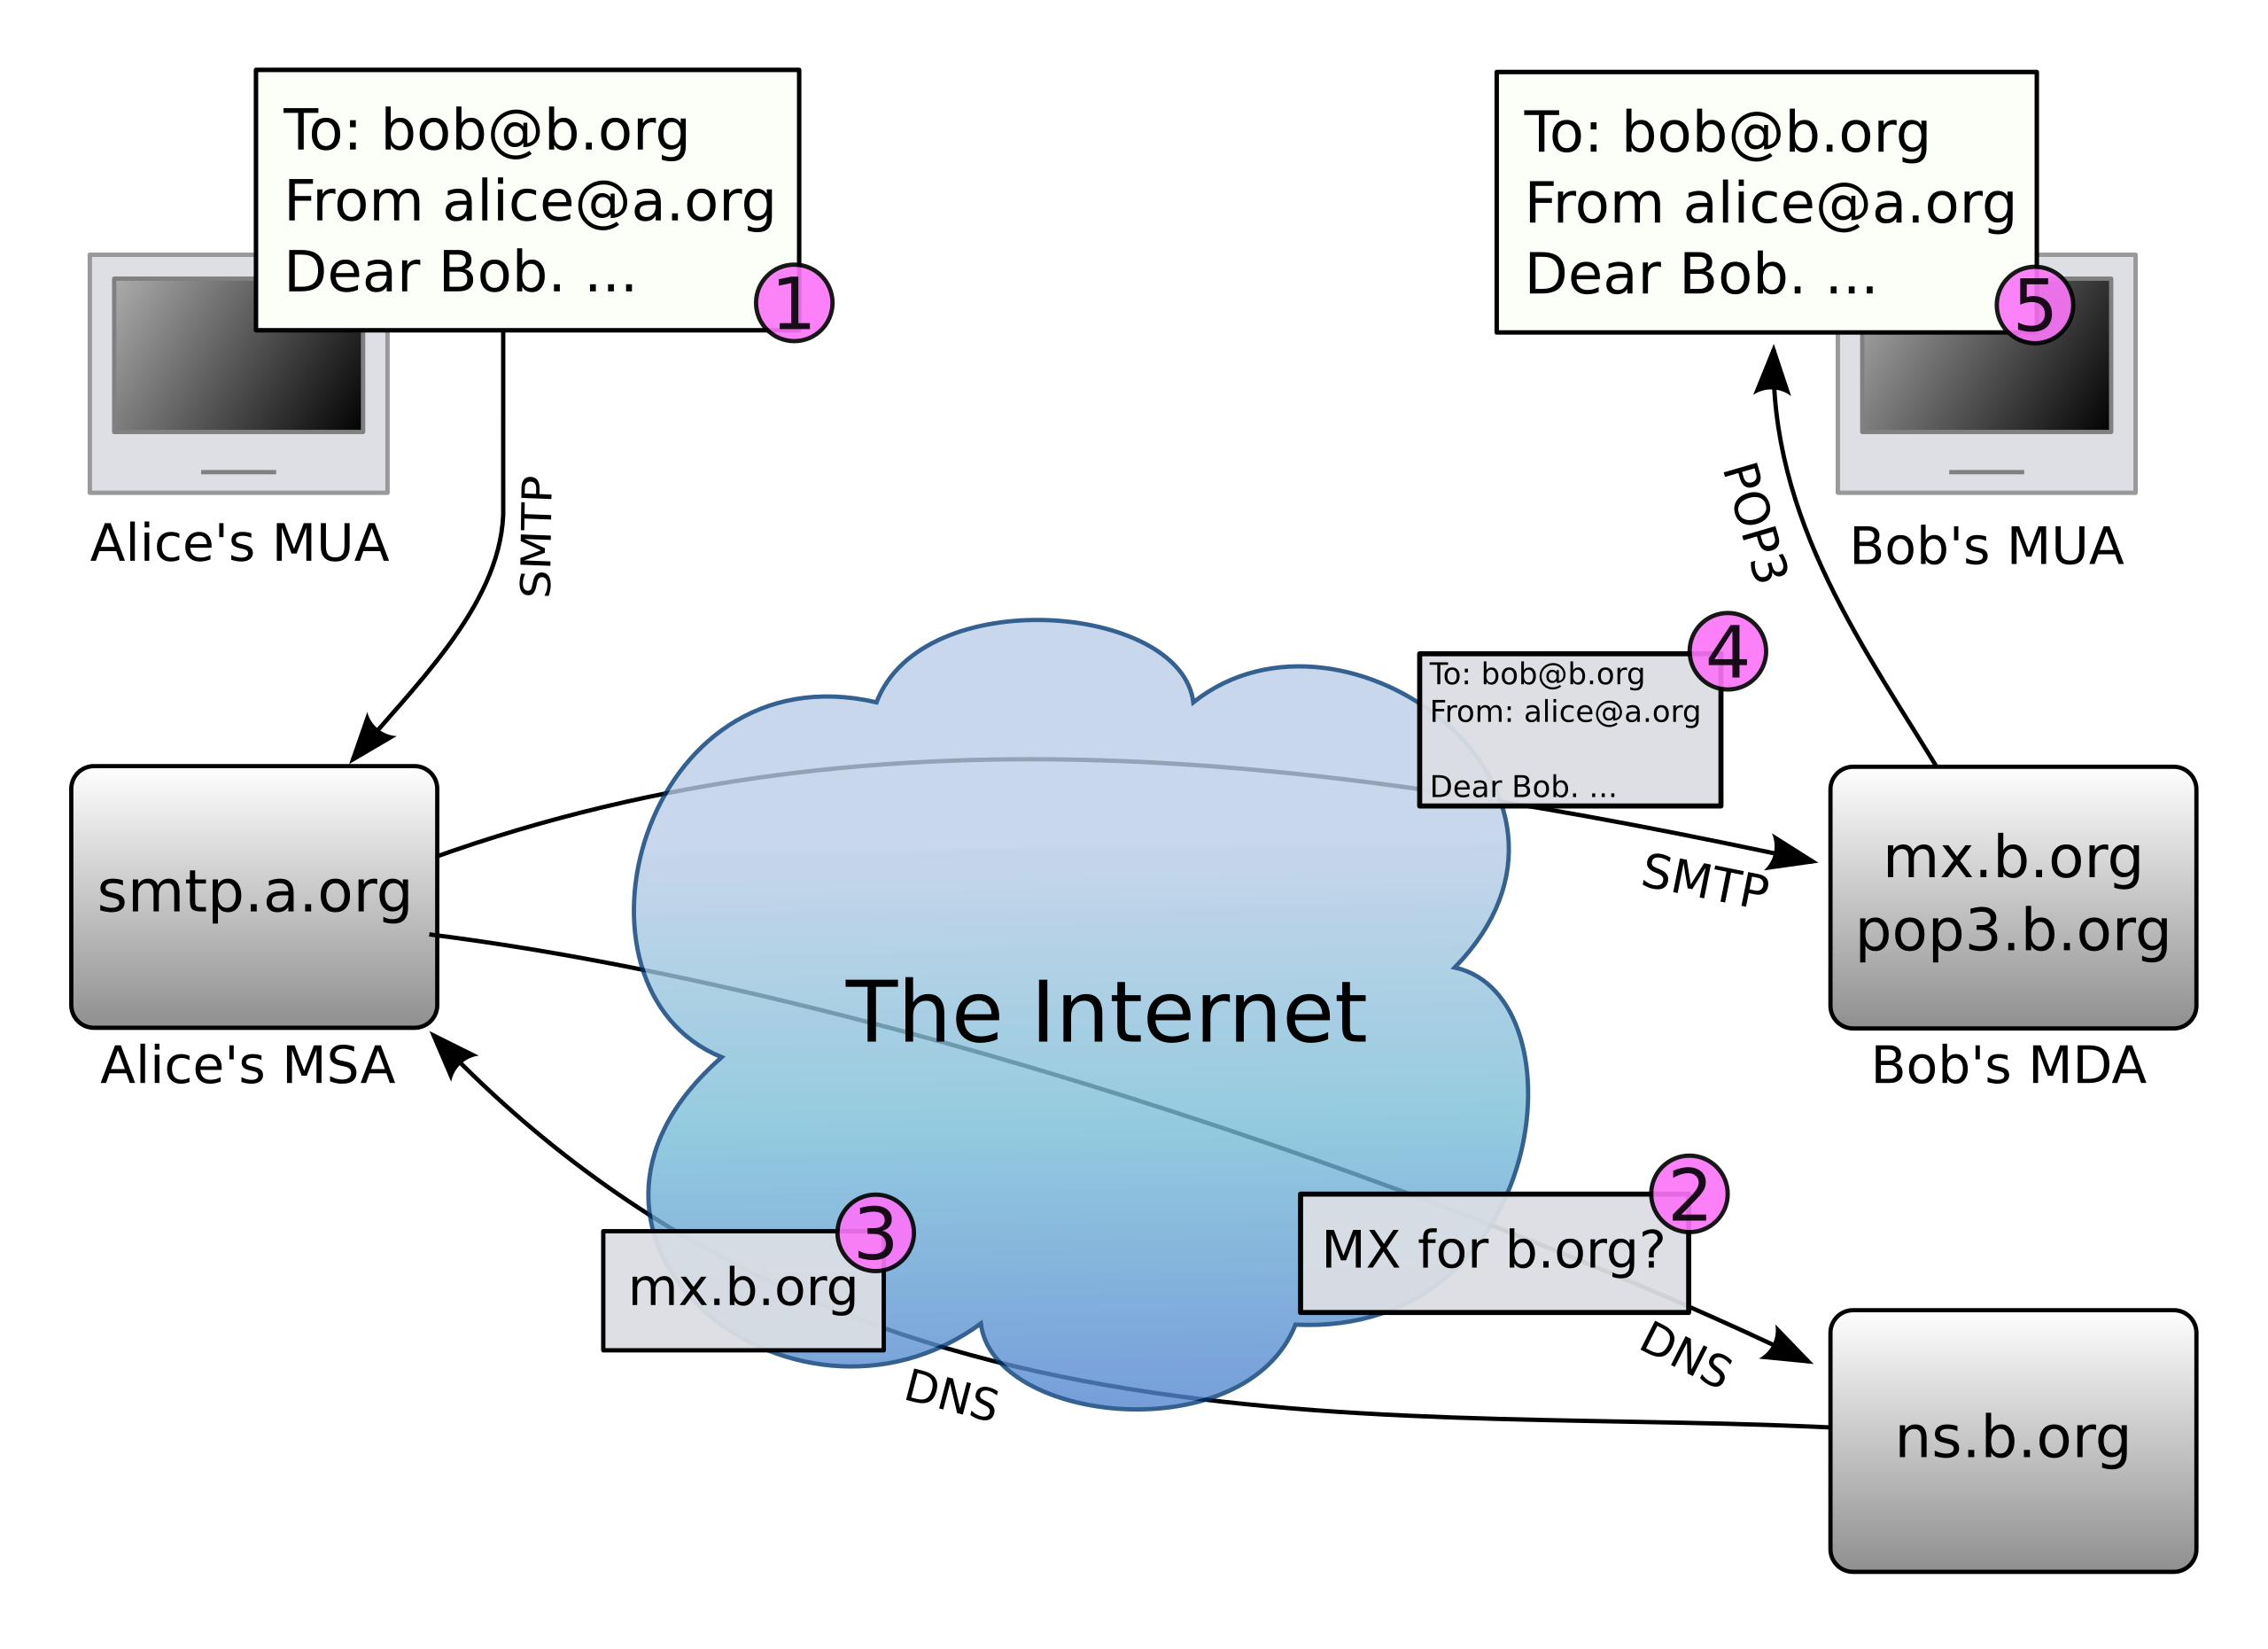
\includegraphics[width=0.8\textwidth]{federated-email}

  % remember to cite the source of the image
  \caption{Arquitetura do \textit{email}, um protocolo federado, que consiste em cada usuário escolher um servidor para ser seu provedor de mensagens. Mensagens entre usuários de servidores diferentes são roteadas pelos próprios servidores. \cite{email-picture}}
\end{figure}

\subsection{\textit{E-Mail}}

O \textit{e-mail} (correio eletrônico) é um sistema de comunicação digital que permite o envio e recebimento de mensagens e arquivos entre usuários através de redes de computadores, utilizando protocolos como \textit{SMTP}, \textit{POP3} e \textit{IMAP} para a transmissão e armazenamento das mensagens. É amplamente utilizado para comunicação pessoal e profissional, sendo uma das formas mais comuns de troca de informações na Internet. \cite{rfc5321}

\begin{itemize}
  \item \textbf{Tipo de endereço}: usuário@servidor
  \item \textbf{Suporte a criptografia de ponta a ponta}: Sim
\end{itemize}

\subsection{\textit{Matrix}}

O protocolo \textit{Matrix} é um sistema de comunicação descentralizado e federado projetado para suportar mensagens instantâneas e colaboração em tempo real. Desenvolvido para ser uma solução aberta e interoperável, o \textit{Matrix} visa fornecer uma infraestrutura robusta para comunicação em diversos contextos, desde \textit{chat} e chamadas de voz até a troca de arquivos. \cite{matrixspec}

\begin{figure}
  \centering
  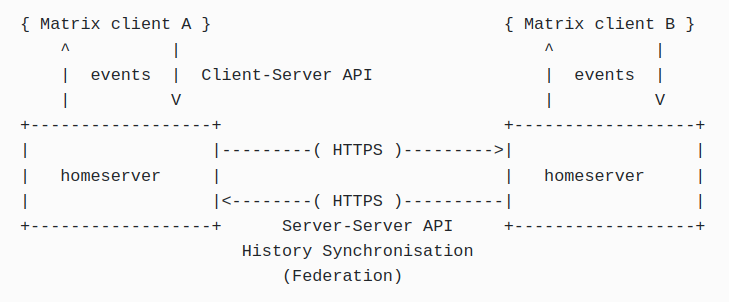
\includegraphics[width=0.8\textwidth]{matrix}

  % remember to cite the source of the image
  \caption{Arquitetura do protocolo \textit{Matrix}, que assim como o \textit{e-mail} consiste em cada usuário escolher um servidor para ser seu provedor de mensagens. Mensagens entre usuários de servidores diferentes são roteadas pelos próprios servidores. \cite{matrixspec}}
\end{figure}

\begin{itemize}
  \item \textbf{Tipo de endereço}: @usuário:servidor
  \item \textbf{Suporte a criptografia de ponta a ponta}: Sim
\end{itemize}

\subsection{\textit{XMPP}}

\textit{XMPP} (\textit{Extensible Messaging and Presence Protocol}) é um protocolo de comunicação em tempo real, baseado em \textit{XML}, que permite a troca descentralizada e segura de mensagens, presença e dados estruturados entre clientes e servidores, suportando uma ampla variedade de funcionalidades, como \textit{chat}, voz, vídeo e colaboração em grupo, sendo reconhecido por sua extensibilidade e interoperabilidade. \cite{xmppspec}

\begin{itemize}
  \item \textbf{Tipo de endereço}: usuário@servidor
  \item \textbf{Suporte a criptografia de ponta a ponta}: Sim
\end{itemize}
\section{Protocolos Peer-to-Peer com \textit{Relays} que não usam \textit{Tor}}

Na arquitetura \textit{peer-to-peer} com \textit{relays}, seja com \textit{Tor} ou não, os usuários se conectam diretamente uns aos outros e armazenam localmente suas mensagens. Para contornar limitações de rede, como camadas de \textit{NAT} e \textit{firewalls}, os usuários podem usar \textit{relays} para intermediar a comunicação. Os \textit{relays} são apenas responsáveis por encaminhar diretamente as mensagens, apagando-as quando elas são entregues. Em alguns protocolos, esses \textit{relays} podem armazenar a mensagem por um curto período de tempo, até o destinatário estar disponível para recebê-la. Os seguintes protocolos utilizam \textit{relays} para intermediar a comunicação entre usuários.

\subsection{\textit{SimpleX}}

O \textit{SimpleX} é um protocolo de mensagens instantâneas \textit{peer-to-peer} que utiliza \textit{relays} para intermediar a comunicação entre usuários. Sua característica distinta é a sua completa ausência de um identificador de usuário, de modo que usuários podem iniciar uma conversa utilizando um simples código de convite. \cite{simplex}

\begin{itemize}
  \item \textbf{Tipo de endereço}: Código de convite
  \item \textbf{Suporte a criptografia de ponta a ponta}: Sim
  \item \textbf{Assíncrono}: Sim
\end{itemize}

\subsection{\textit{IRC}}

O \textit{IRC} (\textit{Internet Relay Chat}) é um protocolo de comunicação em tempo real que foi muito popular no final dos anos 90 e início dos anos 2000, e que ainda é utilizado por algumas comunidades \textit{online}. Neste protocolo, mensagens só podem ser recebidas de forma síncrona, uma vez que o servidor se comporta como um \textit{broadcast}, enviando as mensagens para todos os usuários conectados. \cite{rfc2810}

\begin{itemize}
  \item \textbf{Tipo de endereço}: endereço de servidor
  \item \textbf{Suporte a criptografia de ponta a ponta}: A maioria dos clientes não suporta
  \item \textbf{Assíncrono}: Não
\end{itemize}

\subsection{\textit{LoRaWan}}

O \textit{LoRaWan} é um protocolo de comunicação de longo alcance e baixa potência que permite a comunicação entre dispositivos de \textit{Internet of Things} (\textit{IoT}). O protocolo se utiliza tanto de \textit{LoRa}, que é uma tecnologia de modulação de rádio, quanto de redes de \textit{relays} para transmitir mensagens entre dispositivos pela Internet. \cite{lorawan}

\begin{itemize}
  \item \textbf{Tipo de endereço}: endereço do dispositivo
  \item \textbf{Suporte a criptografia de ponta a ponta}: Sim
  \item \textbf{Assíncrono}: Sim
\end{itemize}

\section{Protocolos Peer-to-Peer com \textit{Relays} que usam \textit{Tor}}

Os seguintes protocolos utilizam a rede do \textit{Tor} para mediar a negociação de chaves e a comunicação entre usuários.

\subsection{\textit{Cwtch}}

O \textit{Cwtch} é um protocolo de mensagens instantâneas \textit{peer-to-peer} que utiliza a rede \textit{Tor} para intermediar a comunicação entre usuários. Cada usuário roda um serviço oculto no \textit{Tor}, e os usuários se conectam diretamente uns aos outros através da rede \textit{Tor}. \cite{cwtch}

\begin{itemize}
  \item \textbf{Tipo de endereço}: Endereço do serviço oculto
  \item \textbf{Suporte a criptografia de ponta a ponta}: Sim
  \item \textbf{Assíncrono}: Não
\end{itemize}

\subsection{\textit{Ricochet}}

O \textit{Ricochet} funciona de maneira muito similar ao \textit{Cwtch}. Cada usuário também roda um serviço oculto, e conecta-se aos serviços ocultos dos outros usuários. \cite{ricochet}

\begin{itemize}
  \item \textbf{Tipo de endereço}: Endereço do serviço oculto
  \item \textbf{Suporte a criptografia de ponta a ponta}: Sim
  \item \textbf{Assíncrono}: Não
\end{itemize}

\subsection{\textit{Briar}}

O \textit{Briar} é um protocolo muito versátil, e que permite o envio de mensagens através de \textit{Bluetooth}, \textit{Wi-Fi}, ou da Internet. Quando as mensagens são enviadas pela Internet, ele utiliza a rede \textit{Tor} para intermediar a comunicação entre usuários, e é capaz de funcionar mesmo em redes censuradas. \cite{briar}

\begin{itemize}
  \item \textbf{Tipo de endereço}: Chave pública e privada (por meio de um \textit{QR code})
  \item \textbf{Suporte a criptografia de ponta a ponta}: Sim
  \item \textbf{Assíncrono}: Sim (com um dispositivo secundário rodando o serviço \textit{Briar Mailbox})
\end{itemize}

\section{Protocolos Peer-to-Peer sem \textit{Relays}}

Na arquitetura \textit{peer-to-peer} sem \textit{relays}, os usuários se conectam diretamente, ou através de outros usuários, mas o protocolo não tem computadores dedicados para o intermédio de mensagens. Em geral, esses protocolos precisam que o usuário inicialmente saiba o endereço de outros usuários para poder se comunicar com eles, e estes protocolos são mais vulneráveis a restrições na rede, como \textit{NATs} e \textit{firewalls}.

\subsection{\textit{Secure Scuttlebutt}}

O \textit{Secure Scuttlebutt} é um protocolo de rede social descentralizada. Nele, os usuários enviam suas postagens diretamente ou indiretamente para outros usuários, sendo assim resiliente a falhas e limitações de rede, e permitindo que usuários acessem conteúdo de forma assíncrona. Para permitir o envio indireto de mensagens ele implementa uma \textit{Epidemic Broadcast Tree} \cite{ebtpaper}, que replica mensagens de usuários para seus amigos na rede. \cite{scuttlebutt}

\begin{itemize}
  \item \textbf{Tipo de endereço}: endereço, porta e chave pública
  \item \textbf{Suporte a criptografia de ponta a ponta}: Sim
  \item \textbf{Assíncrono}: Sim, por meio de replicação de mensagens
\end{itemize}

\subsection{\textit{Tox}}

O \textit{Tox} é um protocolo de mensagens \textit{peer-to-peer} que permite o envio de mensagens de texto, assim como chamadas de voz e vídeo. Enquanto ele não permite o envio indireto de mensagens, ele implementa "\textit{Bootstrap Nodes}", que são máquinas que auxiliam usuários a encontrar a \textit{Tabela de Hash Distribuída} (\textit{DHT}, do inglês) do \textit{Tox}, que é usada para encontrar outros usuários. \cite{toxcore}

\begin{itemize}
  \item \textbf{Tipo de endereço}: Chave pública
  \item \textbf{Suporte a criptografia de ponta a ponta}: Sim
  \item \textbf{Assíncrono}: Não
\end{itemize}

\subsection{\textit{Bitmessage}}

\textit{Bitmessage} é um protocolo que apresenta similaridades com o \textit{Bitcoin}, uma vez que usuários precisam resolver um desafio de prova de trabalho para enviar mensagens. Nele, mensagens percorrem a rede inteira até chegar ao destinatário. \cite{bitmessage}

\begin{itemize}
  \item \textbf{Tipo de endereço}: Chave pública
  \item \textbf{Suporte a criptografia de ponta a ponta}: Sim
  \item \textbf{Assíncrono}: Sim
\end{itemize}